    \documentclass[letterpaper,11pt]{article}

    \usepackage{fullpage}
    \usepackage[usenames,dvipsnames]{color}
    \usepackage[pdftex]{hyperref}
    \usepackage{tabularx}
\usepackage{booktabs}
\usepackage{amsmath}
\usepackage{multirow}
\usepackage{layouts}
\usepackage{array}
\usepackage{pgf}
\usepackage{tikz}
\usetikzlibrary{positioning}
\usetikzlibrary{arrows,automata}
 \usepackage{graphicx}

    \hypersetup{
	colorlinks,%
	citecolor=black,%
	filecolor=black,%
	linkcolor=black,%
	urlcolor=mygreylink     % can put red here to visualize the links
    }
   
    \definecolor{mygrey}{gray}{.85}
    \definecolor{mygreylink}{gray}{.30}
    \textheight=8.6in
    \raggedbottom
    \raggedright
    \setlength{\tabcolsep}{0in}
    \addtolength{\oddsidemargin}{-0.375in}
    \addtolength{\evensidemargin}{0.375in}
    \addtolength{\textwidth}{0.5in}
    \addtolength{\topmargin}{-.375in}
    \addtolength{\textheight}{0.75in}

    \newcommand{\resitem}[1]{\item #1 \vspace{-2pt}}
    \newcommand{\resheading}[1]{{\large \colorbox{mygrey}{\begin{minipage}{\textwidth}{\textbf{#1 \vphantom{p\^{E}}}}\end{minipage}}}}
    \newcommand{\ressubheading}[4]{
    \begin{tabular*}{6.5in}{l@{\extracolsep{\fill}}r}
		    \textbf{#1} & #2 \\
		    \textit{#3} & \textit{#4} \\
    \end{tabular*}\vspace{-6pt}}
  
    \begin{document}

\begin{center}
{\LARGE \textbf{Machine Learning: Pattern Recognition}}\\ [1em]
\end{center}
\newcommand{\mywebheader}{
    \begin{tabular}{@{}p{5in}p{4in}}
		{\resheading{Report Lab 1}} & {\Large 11 September, 2012}\\\vspace{0.2cm}
	    \end{tabular}}
    \mywebheader
    
    	\begin{center}
    	{\Large By:} \\ \vspace{0.1cm}
	    {\Large Paris Mavromoustakos} \\  \vspace{0.1cm}
	    {\Large Georgios Methenitis} \\ \vspace{0.1cm}
	    {\Large Marios Tzakris}
	    \end{center}

  
  \section*{Introduction}
  The purpose of this lab assignment was to apply a k-Nearest-Neighbours classification algorithm on a given set of datapoints. To achieve this we had to become familiar with the Matlab environment, including the Netlab package. The Netlab package is a complete suit of matlab functions implementing machine learning techniques.
 
 \section*{Exercise 1}
 First of all, we loaded a given data file (twoclass.mat) which contained two classes of two-dimensional datapoints. Before creating both the training and test sets, we shuffled the two matrices in order to create groups of random datapoints. \textbf{The training set consists of 75\% of class A's datapoints appended to 75\% of class B's datapoints, while the test set contains the remaining 25\% of both classes}. Figure \ref{fig:1} presents the plot results of the training set. \textbf{Datapoints of different classes are depicted with different symbols and colors}. Figure \ref{fig:2} presents the plot results of the test set.
 
 \begin{figure}[h!]
\centering
  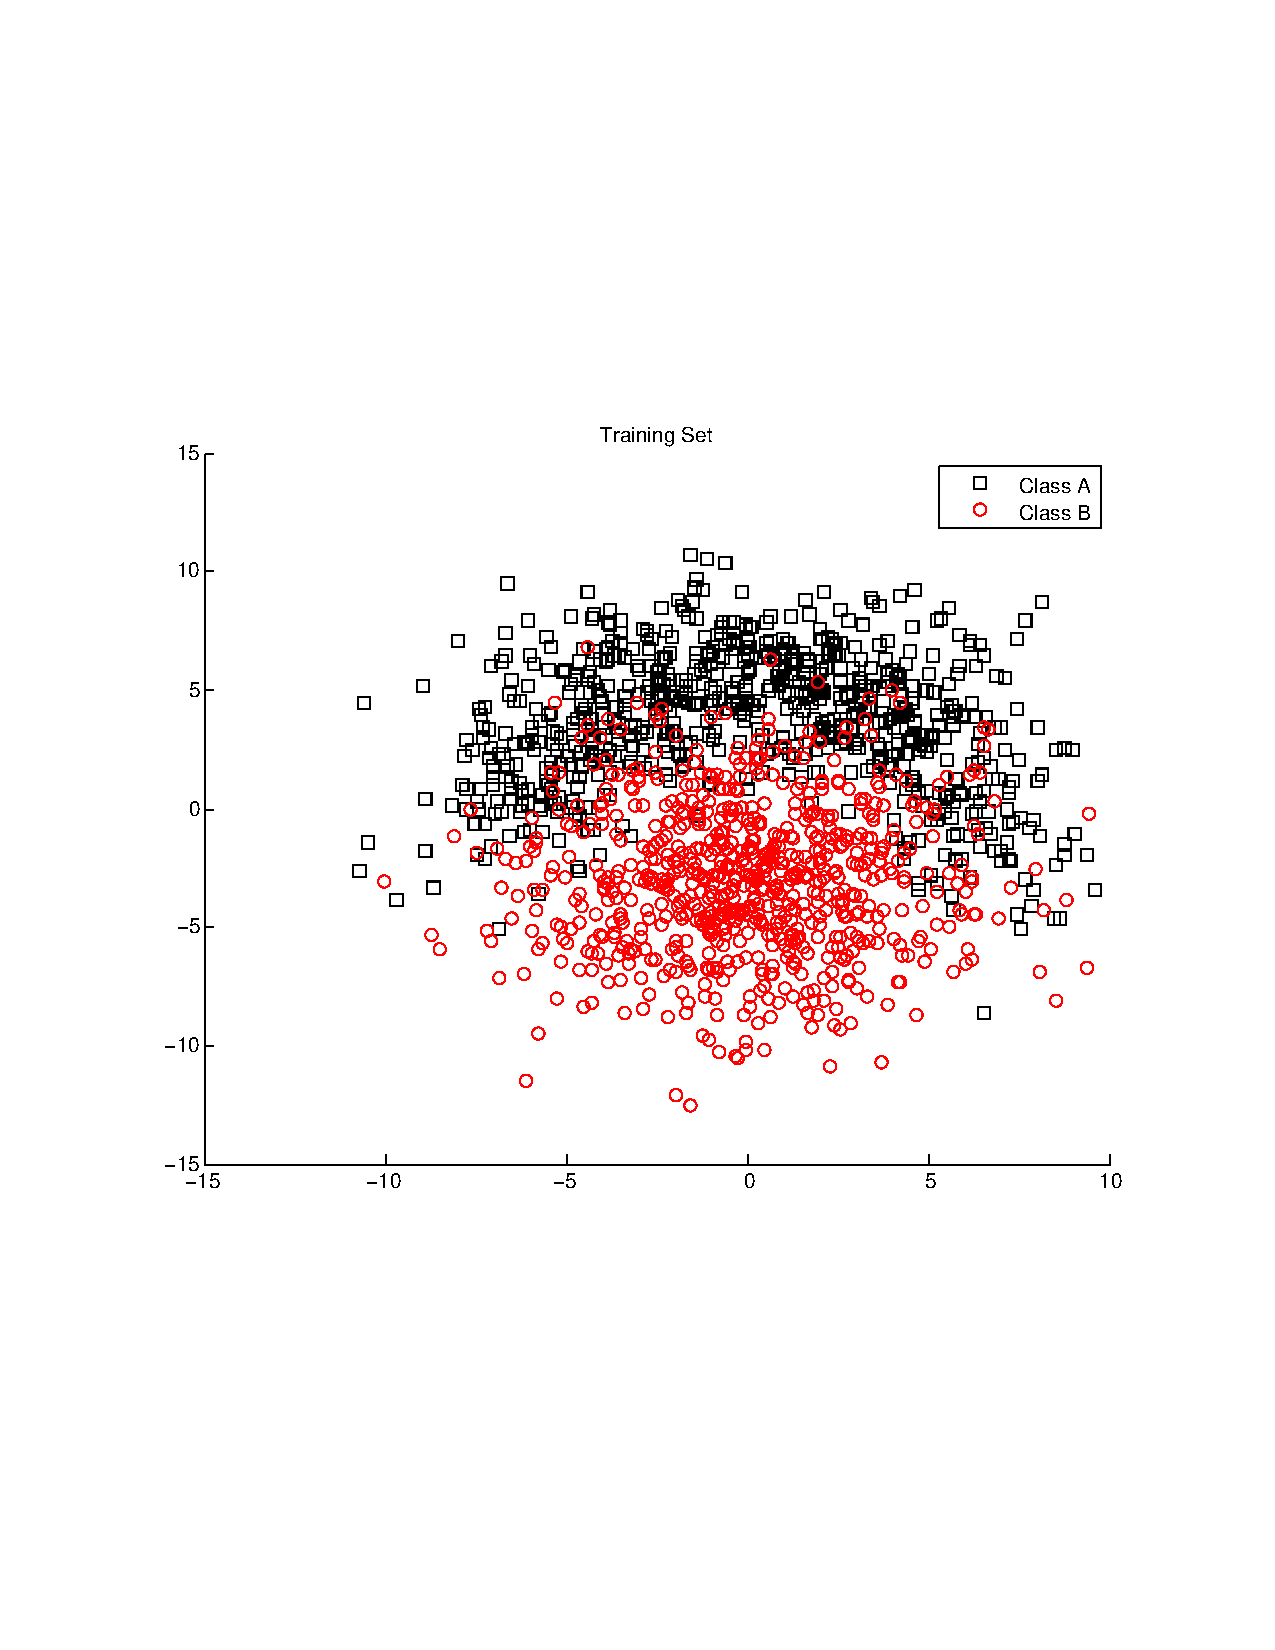
\includegraphics[trim = 0cm 7.5cm 0cm 7.5cm, clip, width=0.8\textwidth]{figures/TrainingSet.pdf}
  \caption{Training Set.}
  \label{fig:1}
\end{figure}
 
  \begin{figure}[t!]
\centering
  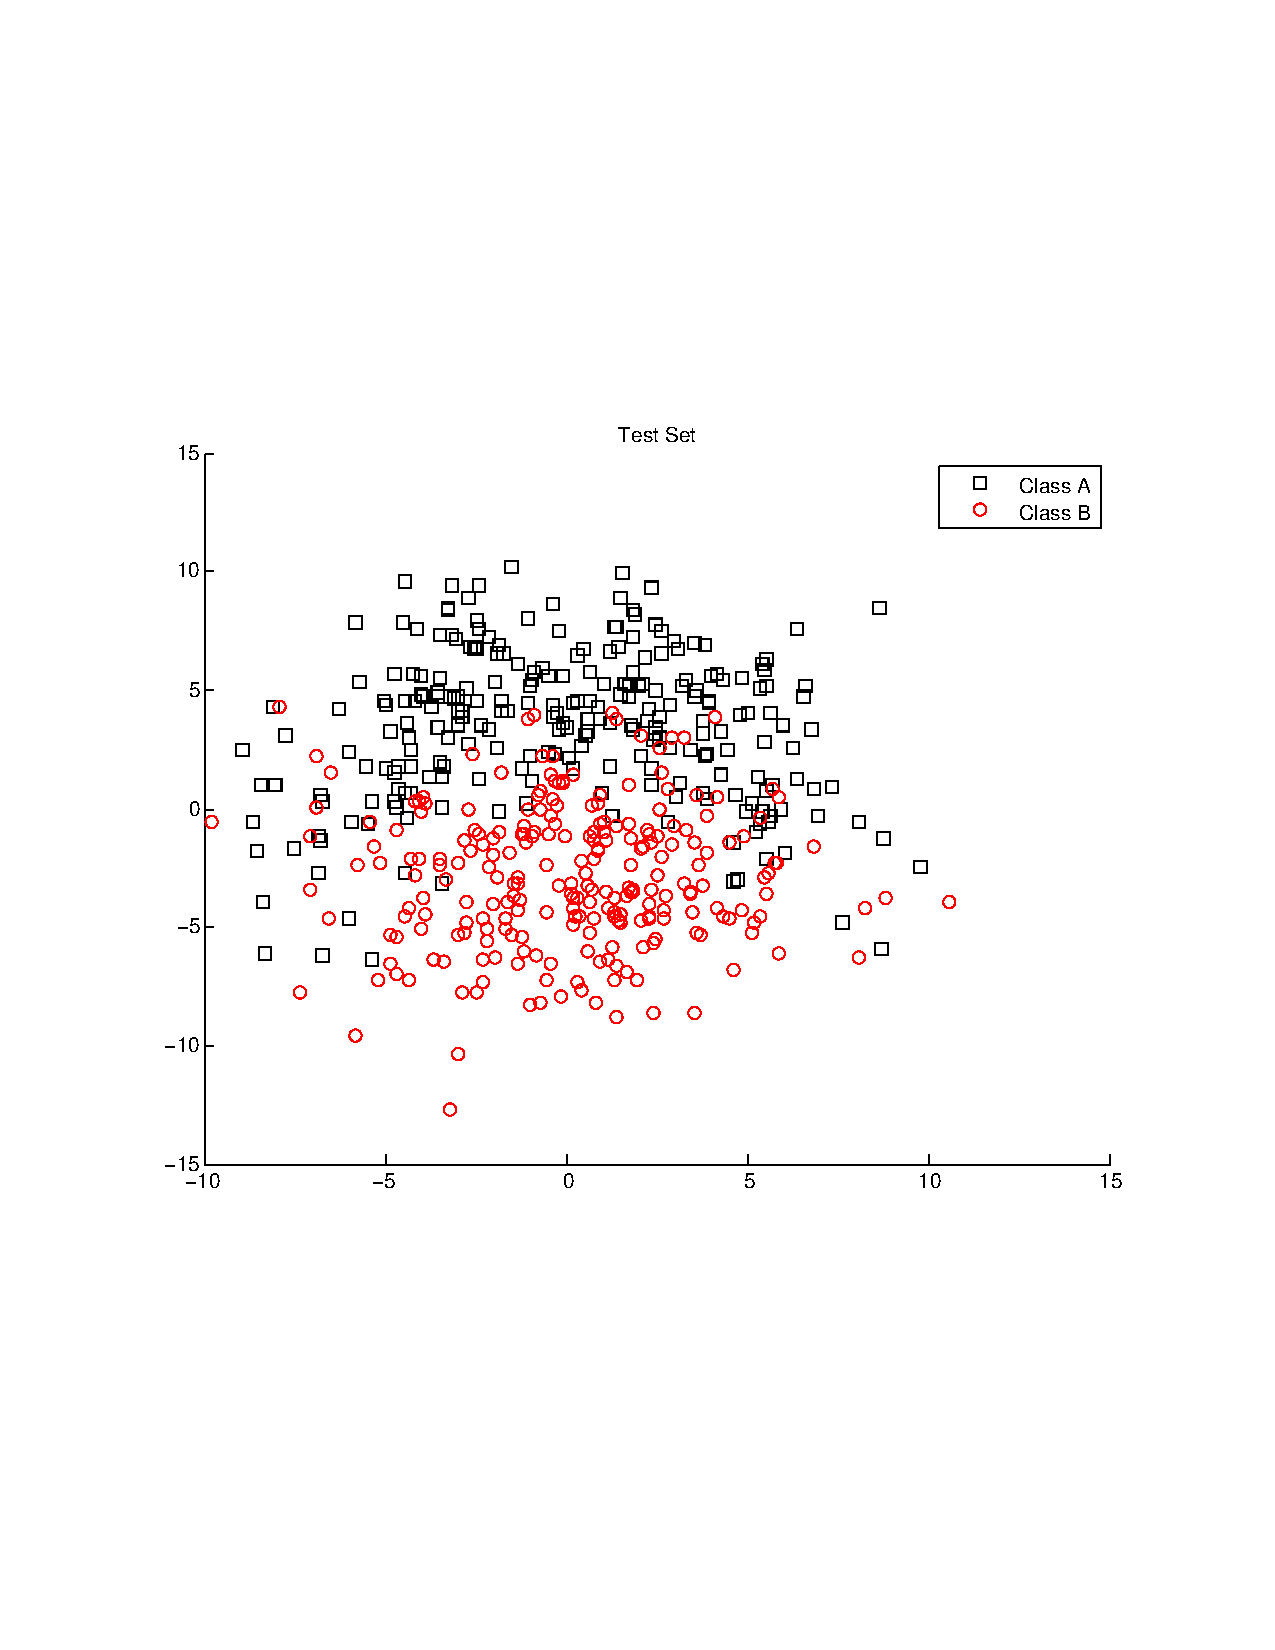
\includegraphics[trim = 0cm 7.5cm 0cm 7.5cm, clip, width=0.8\textwidth]{figures/TestSet.pdf}
  \caption{Training Set.}
  \label{fig:2}
\end{figure}



\section*{Exercise 2}
We trained our knn classifier using the training data, evaluating its performance on the test data and computing the misclassification rate. The misclassification rate taking into consideration only one neighbour (k=1) is 17\%. Then we tried several odd values for k (k=1, 3, 5, \ldots, 29), computing the error for each case as shown in Figure \ref{fig:3}.


  \begin{figure}[h!]
\centering
  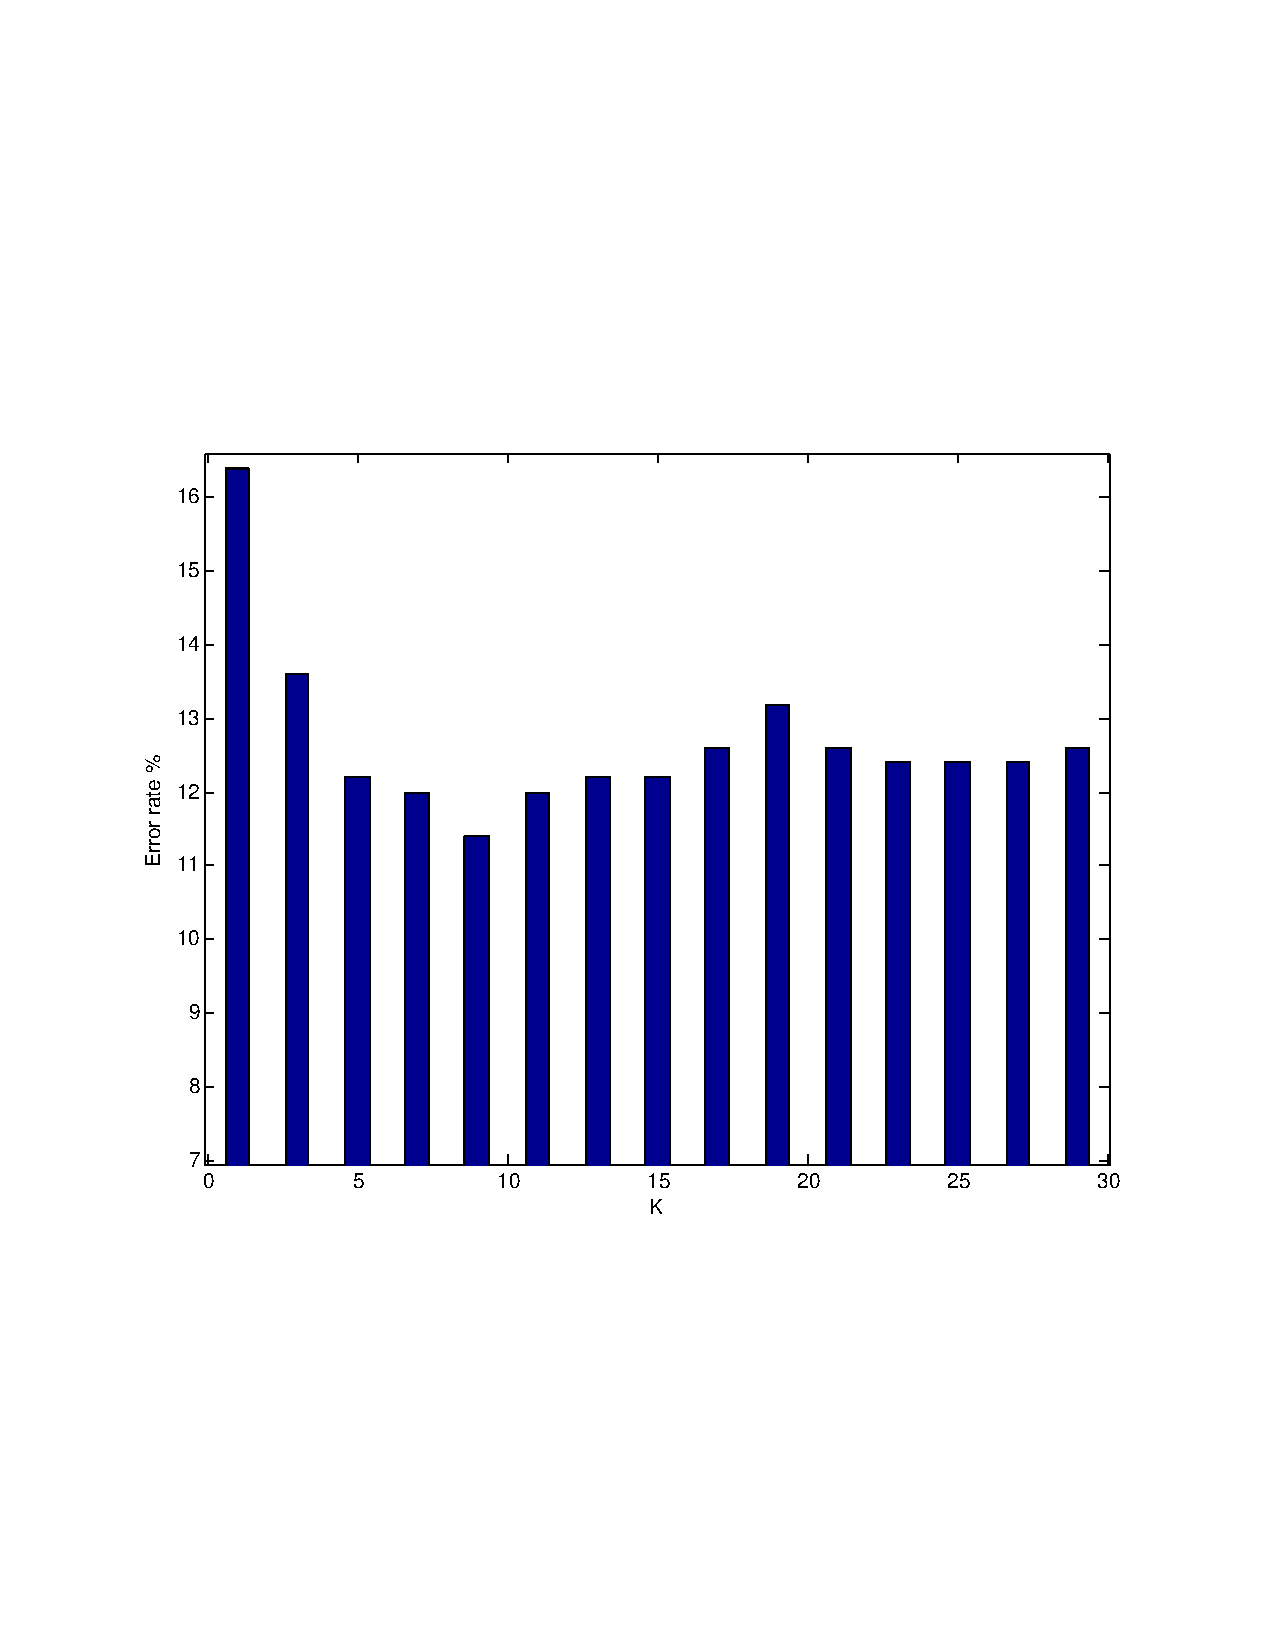
\includegraphics[trim = 0cm 7cm 0cm 7.5cm, clip, width=0.8\textwidth]{figures/KnnResults.pdf}
  \caption{Classification Results.}
  \label{fig:3}
\end{figure}

The value of k that we would choose is \textbf{k=9}, because as the figure states, for k=9 the \textbf{test error} reaches its \textbf{minimum} value, however, for $k>9$, an incrementation of the misclassification rate is detected as we increase the value of k. However, we are not able to definately state that k=9 is the optimal value for k. As mentioned above, as the value of k increases, the test error is expected to decrease. This behavior does not refer to the whole range of k's tested values, but as k becomes significantly high the test error calculated increments aswell. We interpreted this fact as a typical case of \textbf{overfitting}, which is \textbf{expected} to occur if the value of k becomes high enough (in this case, $k>9$).



 \section*{Exercise 3}
As described before, an \textbf{overfitting} problem has occurred while increasing the value of k. This might happen because either we have a model which is too complex, or the data used for training is too little. In our case, the model is relatively simple so, we should find a way to increase our training data. Here comes the solution of \textbf{cross-validation}. Cross-validation helps overcome overfitting while \textbf{expanding the data used for training purposes}. Each time we run the algorithm, a new training and test set is being used, thus giving us more \textbf{accurate predictions} when it comes to validation. Another algorithm we could apply in order to increase accuracy, is \textbf{bootstrapping}, which would at least lead us to a critical conclusion regarding the variance of the data we were given, informing us about the possible outcome of the whole simulation.
We applied cross-validation not onty to expand our training and test data, but also to reach a more \textbf{reliable conclusion} about the value of k. 


\begin{figure}[!h]
\centering
  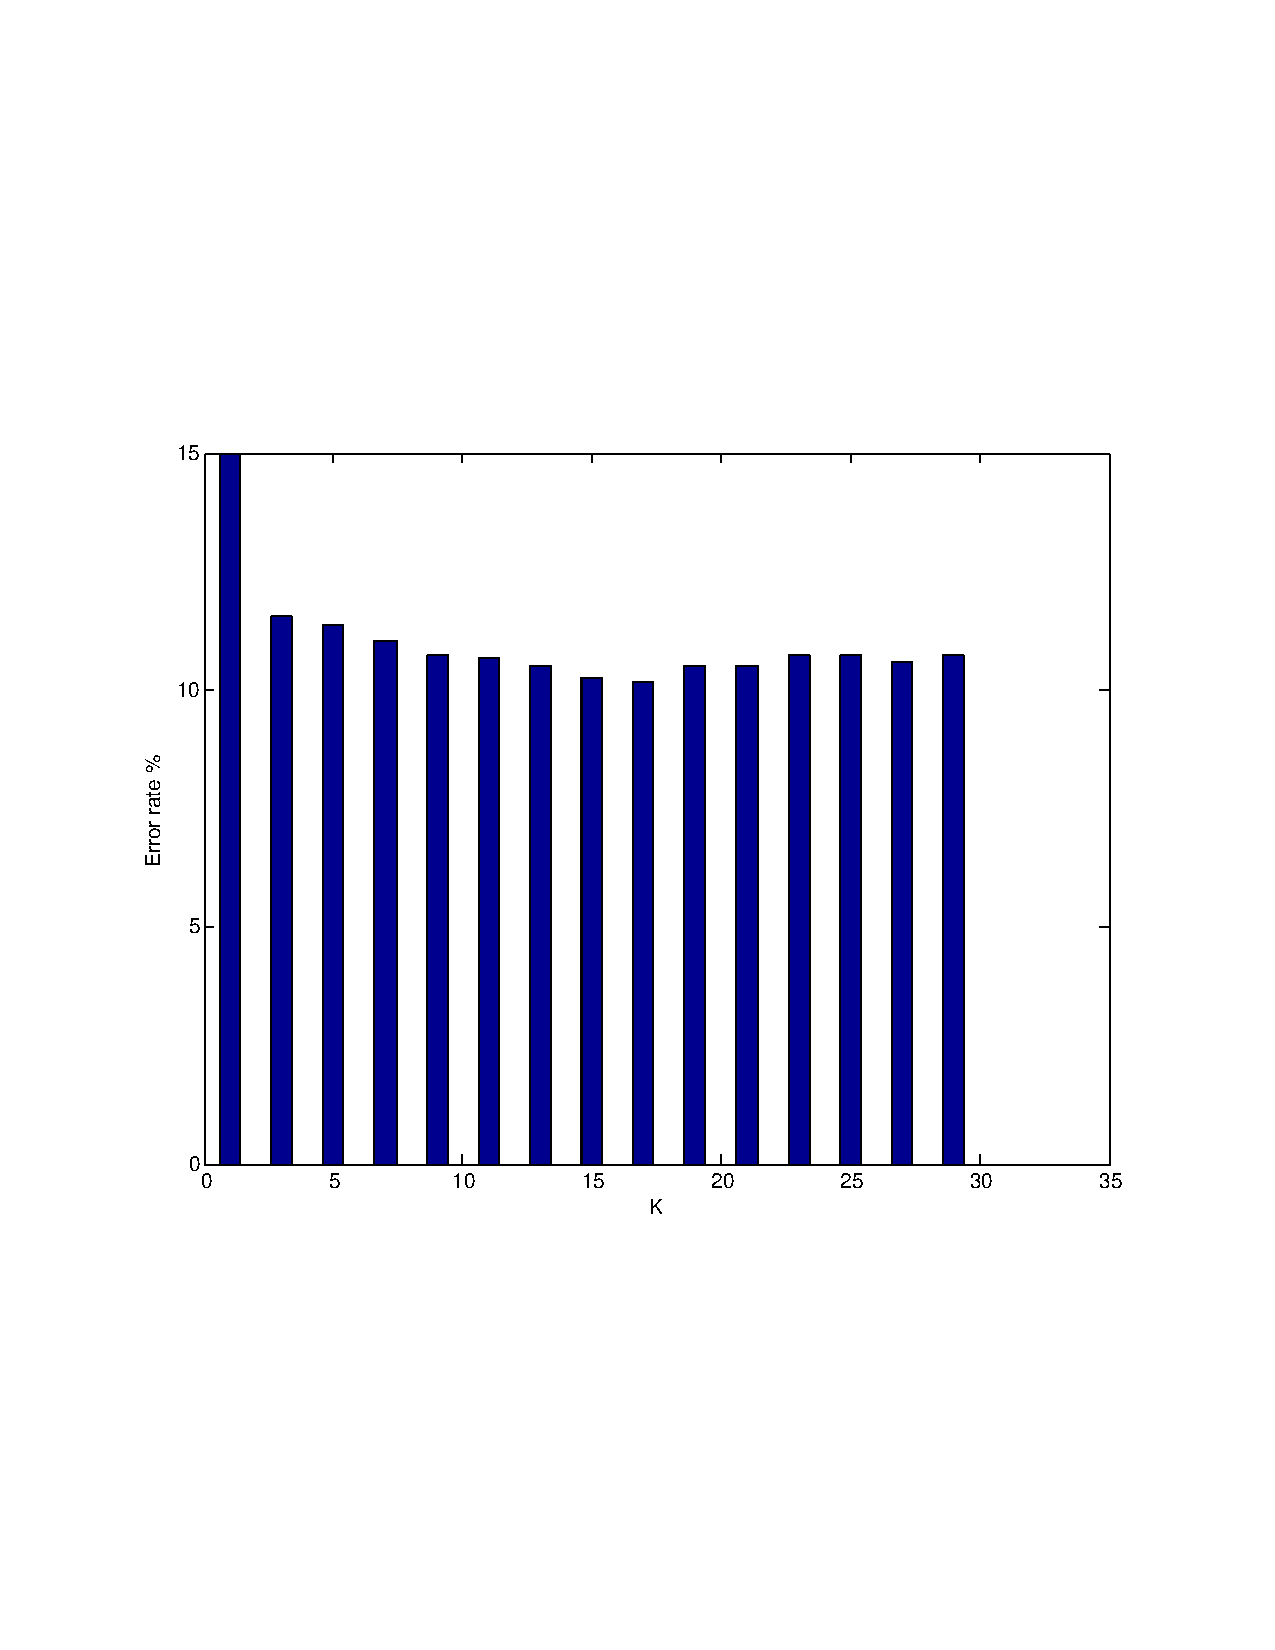
\includegraphics[trim = 0cm 7cm 0cm 7.5cm, clip, width=0.8\textwidth]{figures/CrossValResults.pdf}
  \caption{Results of Cross-Validation}
  \label{fig:4}
\end{figure}



As shown in Figure \ref{fig:4}, the misclassification error of the cross-validated data reaches its minimum value for k=9, enabling us to state in \textbf{certainty} that k=9 is the optimal value for k.
This value is the one we would use in our \textbf{final classifier}, although the misclassification rate becomes minimum when k=17. We have chosen k=9 because we prefer to "sacrifice" a very small difference in the algorithm's \textbf{accuracy} in order to implement a more \textbf{simple} classificator. We estimated that a value of k=17 would oversmooth our classificator and make our algorithm \textbf{computationally expensive}.
To compute the \textbf{test error}, we calculated the \textbf{average} over the 10 iterations of the 10-fold Cross-Validation algorithm. The test error computed is different in each iteration, so the \textbf{average} value gives us a good estimate of the misclassification error value.
The use of a \textbf{validation set} is to define whether the classificator's predictions are accurate or not.


 


 \section*{Conclusion}
In conclusion, this project has clearly helped us understand the nature of the k-NN algorithm. Moreover, we were able to point out its advantages while facing the expected drawbacks, like the overfitting phenomenon. On the other hand we studied and implemented methods of dealing with overfitting, and thus reaching more accurate and reliable conclusions.


    \end{document}


